\documentclass{myproject}

\graphicspath{{../Figures/}}

% title setup
\title{\vspace*{-1cm}Numerical Analysis of Burgers' Equation\footnote{Placeholder title!}}
\date{}
\author{
    Andre Gormann\\
    agormann@sfu.ca
    \and
    Ethan MacDonald\\
    jem21@sfu.ca
}

% bibliography
\addbibresource{references.bib}

\renewcommand*{\thefootnote}{[\arabic{footnote}]}

\begin{document}

% title creation
\maketitle

% document 
\section{Introduction\protect\footnote{This entire section has been modified from the content in Chapter 2 of \cite{choksi2022}. Specifically, sections 2.2-2.4.}}

\subsection{The Inviscid Burgers' Equation}

We have elected to study the Burgers' equation, or more correctly, the inviscid Burgers' equation.\footnote{We may decide later on to study the viscous Burgers' equation.} Given $u \in C^1(\Omega)$, where $\Omega \subset \R^{n+1}$ is a domain, the general form is written as
\begin{equation}
    \partial_t u(\bm{x},t) + u(\bm{x},t)\cdot \nabla_{\bm{x}} u(\bm{x},t) = 0
\end{equation}
where $ \nabla_{\bm{x}} $ denotes the gradient with respect to the spatial variable $ \bm{x} \in \R^n $. For pragmatic reasons though, we will be focusing on the $n=1$ case. Then (1) simplifies to
\begin{equation}
    \partial_t u(x,t) + u(x,t)\partial_xu(x,t) = 0.
\end{equation}
There are two key observations to make. The first is that (2) is really a statement about the directional derivative, that is
\begin{equation}
    \nabla u(x,t)\cdot (u(x,t), 1) = 0\footnote{Technically we should be normalizing so that this is a unit vector.}
\end{equation}
so the derivative of $u$ in the direction of $(u, 1)$ is 0 - in other words, $u$ is constant in this direction. This is a consequence of (2) being first-order. While on the surface it may seem problematic that (2) is quasilinear (and so the direction $(u, 1)$ is varied), this does not complicate the finding of an analytic solution. 

\subsection{The Method of Characteristics}

Given data on some curve $ \Gamma \subset \overline{\Omega} $, we are looking specific parametric curves $ (x(t), t) $ which connect points $(x, t) \in \Omega$ to $ \Gamma $. We want these curves to be precisely those which are parallel to the vector $(u, 1)$, that is
\[
    \frac{dx}{dt} = \frac{u(x(t), t)}{1} = u(x(t), t)
\]

Now supposing that $u$ solves (2), let $z(t)$ denote the value of $u$ along a characteristic, i.e. 
\[
    z(t) = u(x(t), t)
\]
Then by the chain rule
\[
    \frac{dz}{dt} = \partial_x u(x(t), t) \frac{dx}{dt}u(x(t), t) + \partial_t u(x(t), t)
\]
but $ x'(t) = u(x,t) $, so
\[
    \frac{dz}{dt} = \partial_t u(x(t), t) + u(x,t)\partial_x u(x(t), t)
\]
which is precisely 0 by (2). Hence, we have the following coupled system of ODEs
\begin{equation}
    \begin{cases}
        x'(t) = z(t) = u(x(t), t) \\
        z'(t) = 0
    \end{cases}
\end{equation}
Integrating the second term, we get that
\[
    z(t) = z_0
\]
for some $ z_0 \in \R $. But $z(t) = u(x(t), t)$, so then $u(x(t), t) = z_0$. This corroborates our findings with (3). Now by integrating the first term, we get
\begin{equation}
    x(t) = z_0t + x_0
\end{equation}
where $ x_0 \in \R $. Evaluating at $t=0$, we have that $x(0) = x_0$. Now assuming we are prescribed some initial condition $u(x,0) = g(x)$, we have that (5) becomes
\begin{equation}
    x(t) = g(x_0)t + x_0
\end{equation}
which are exactly those characteristic curves we initially sought.

\subsection{Interpretation}

\begin{figure}
    \centering
    \begin{subfigure}{.48\textwidth}
        \centering
        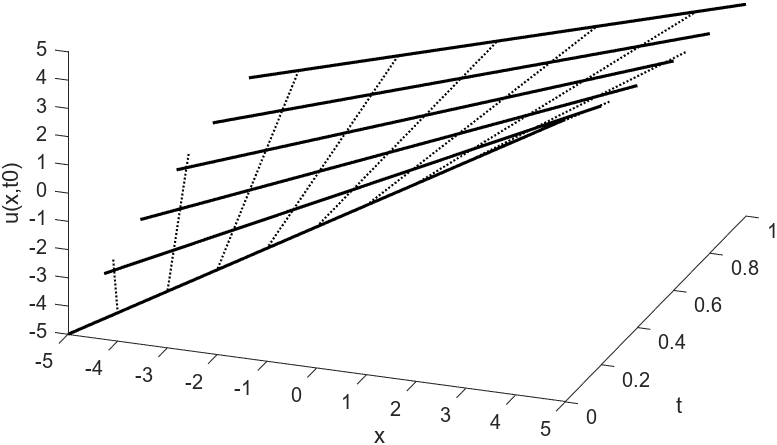
\includegraphics[width=1.0\textwidth]{intro_f1_3d.png}
        \caption{Plot of solution curves at fixed $t\in[0,1]$ with increments of $0.2$.}
        \label{fig:f1_3d}
    \end{subfigure}\hfill
    \begin{subfigure}{.48\textwidth}
        \centering
        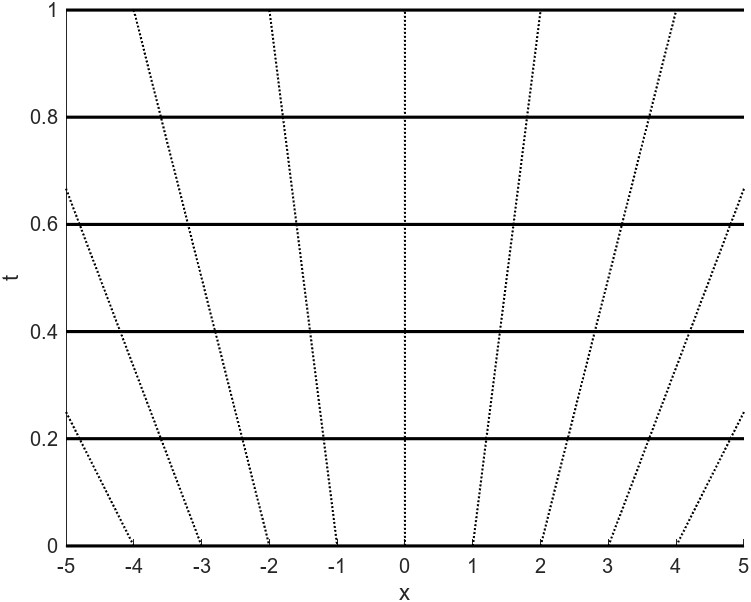
\includegraphics[width=0.75\textwidth]{intro_f1_char.png}
        \caption{Characteristic curves (see (6)) at fixed $x_0 \in [-5, 5]$ with increments of $1$.}
        \label{fig:f1_char}
    \end{subfigure}
    \caption{Solution to (2) with the non-decreasing initial condition $u(x,0) = x$.}
    \label{fig:f1}
\end{figure}

\begin{figure}
    \centering
    \begin{subfigure}{.48\textwidth}
        \centering
        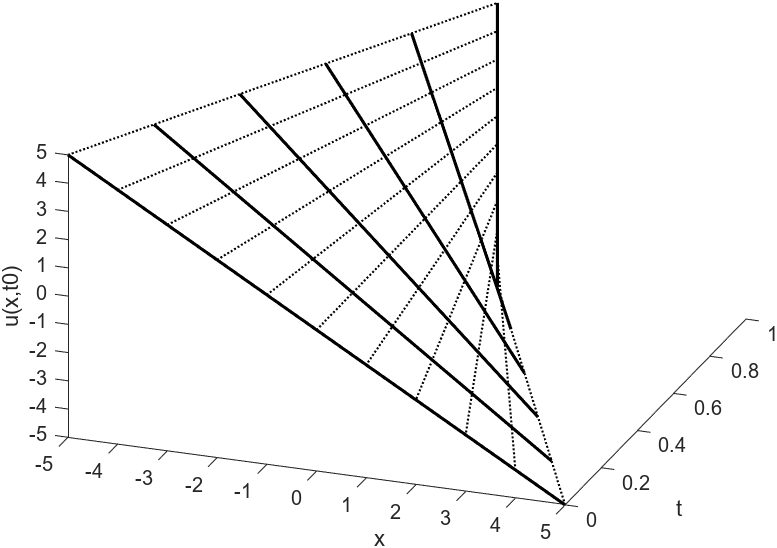
\includegraphics[width=1.0\textwidth]{intro_f2_3d.png}
        \caption{Plot of solution curves at fixed $t\in[0,1]$ with increments of $0.2$.}
        \label{fig:f2_3d}
    \end{subfigure}\hfill
    \begin{subfigure}{.48\textwidth}
        \centering
        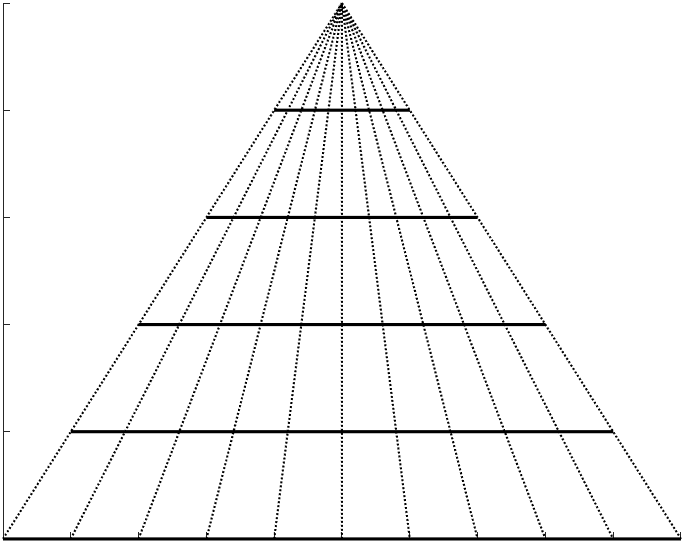
\includegraphics[width=0.75\textwidth]{intro_f2_char.png}
        \caption{Solution to (2) with the non-decreasing initial condition $u(x,0) = x$.}
        \label{fig:f2_char}
    \end{subfigure}
    \caption{Solution to (2) with the initial condition $u(x,0) = -x$.}
    \label{fig:f2}
\end{figure}

\section{Numerical Analysis}

\section{Conclusion}

% bibliography
\nocite{choksi2022}
\nocite{kutz2013}
\printbibliography

\end{document}